\chapter{Introduction}

\section{Motivation}

The idea for this application started with a project developed during a LigaAC LABS laboratory, based on image
processing techniques. Several filters were to be applied onto a raw image file, filters such as blurring,
sharpening and edge detection.

\begin{figure}[H]
	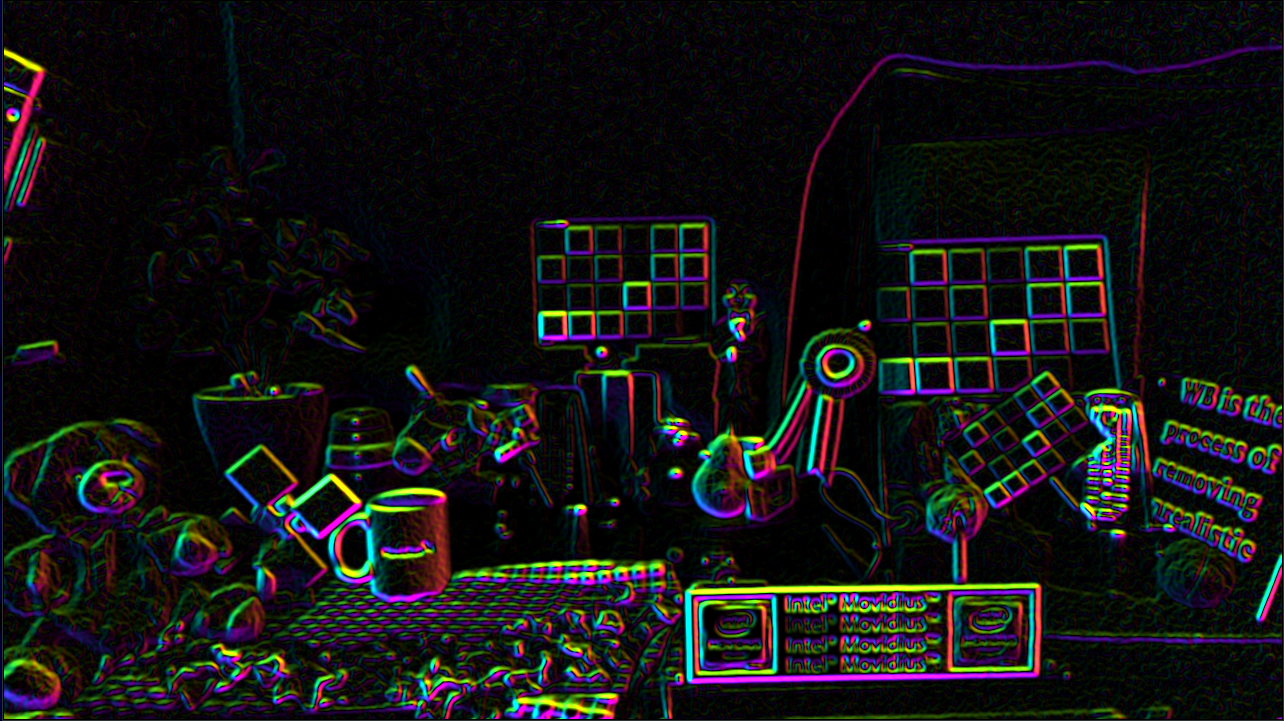
\includegraphics[width=0.9\textwidth, height=0.6\textwidth]{resources/LABS.jpg}
	\caption{Edge detection project for LigaAC LABS}
\end{figure}

From this, the notion arose that each parameter of the aforementioned filters could be tweaked in order to
observe changes in the final output, a process that was quite inefficient due to those parameters being
accessible only during build time.

Thus, the idea for an application that will provide precisely this functionality emerged, with the target 
of presenting several image filters with great visual impact, allowing for each to be modified in order to 
asses the weight of each parameter, packed into a portable package that could be used to showcase image 
processing techniques in the context of various classes and conferences.

\section{Result}

The application went through several design iterations, first of which was the idea of manually accessing an
image, performing several processing steps, then displaying the result. This approach, however, proved to be an 
inefficient process, both in terms of development time, as well as code optimizations. For this reason, an API
that could provide the image loading and displaying functionality, as well as some optimized filters was chosen,
in the form of OpenCV.

This next prototyping hurdle was the need of a user interface. The OpenCV HighUI module was briefly considered,
but was abandoned due to the technical limitations it would impose on the final project. A dedicated user
interface API was required, and for this purpose the QtFramework was chosen, mainly due to its compatibility
with OpenCV.

The graphical interface also suffered several design modifications along its development, with the final design
being centered around the ability to change both the filter parameters, as well as the size and position onto
the initial image that will be affected. The final version of the ISP Demo provides a tool for applying various
image filters, combining different processing steps and allows for the tweaking of all relevant parameters, as
well as the affected area, being most useful when doing a before and after comparison.

\begin{figure}[H]
	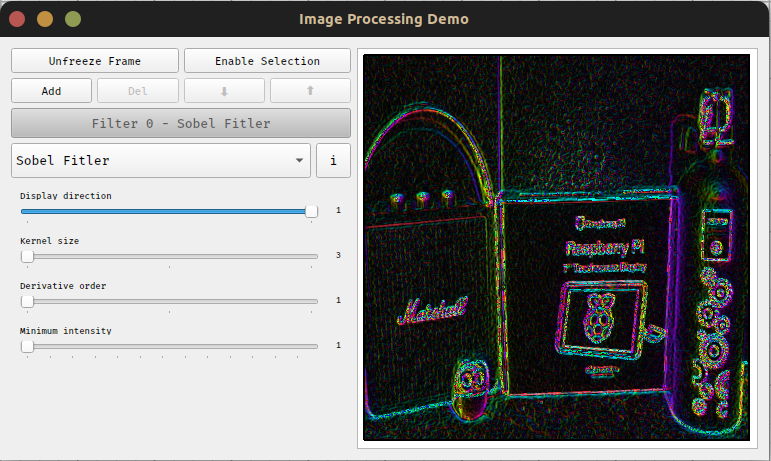
\includegraphics[width=0.9\textwidth, height=0.6\textwidth]{resources/Sobel_5.png}
	\caption{Edge detection result from ISP application}
\end{figure}

